
\section{Usage}
\label{sec:usage}

\begin{figure*}
  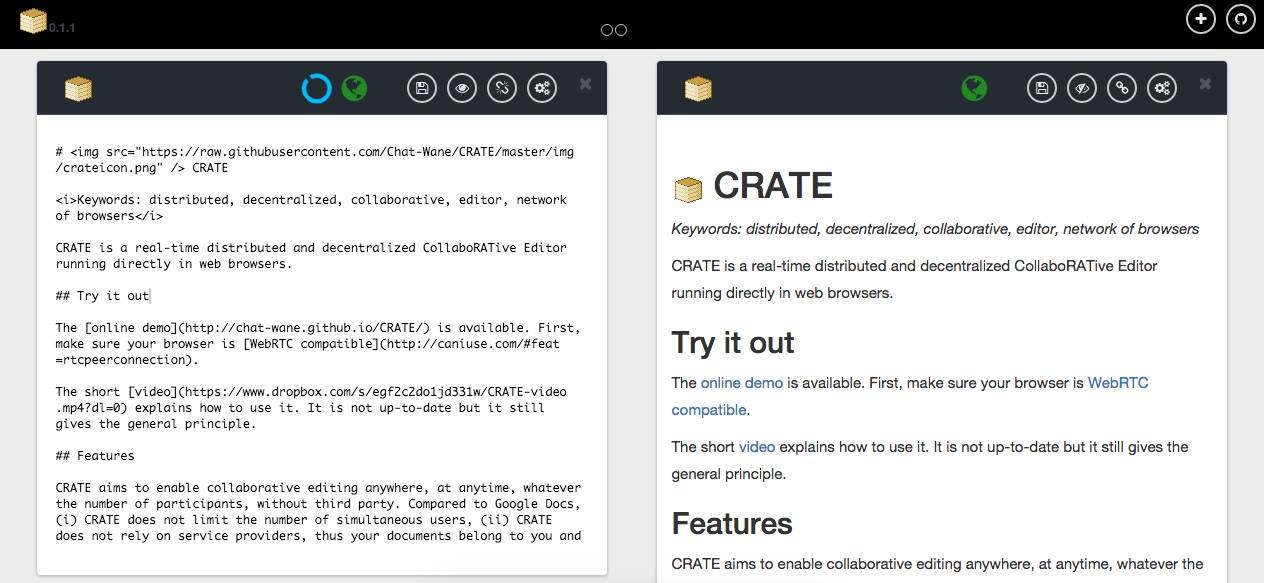
\includegraphics[width=\textwidth]{./img/screenshot.png}
  \caption{\label{img:screenshot} Screenshot of the web application containing
    two editors: on the left, a document is written in markdown language which
    is previewed on the right editor.}
\end{figure*}

\CRATE video, source code and online demo is freely available at
\url{https://github.com/Chat-Wane/CRATE}.

% \CRATE is a real-time collaborative editor running in web browsers accessible on
% the Github plateform at \emph{\url{http://chat-wane.github.io/CRATE/}}. Users
% simply navigate to the web page with their web browser\footnote{The browser must
%   support WebRTC.}.

In the online demo\footnote{\url{http://chat-wane.github.io/CRATE/, the
    browser must support WebRTC}}, a user creates a document by
clicking the $+$ icon at the top the screen (see
Figure~\ref{img:screenshot}). At the time, the document is only local
and no one can read or modify it apart from its creator. When the user
is ready to share, it clicks on the $chain$ icon and \CRATE is
crafting an editing session URL that can be sent by mail, or published
on twitter etc.

Once the collaborators open the link, it automatically connects them
to the editing session of the creator. It retrieves the shared
document and they can start the real-time collaborative editing. In
turn, they are able to share the access to the document too. 

Figure~\ref{img:screenshot} shows a screenshot of the graphical user interface
of \CRATE. In this scenario, two editors are running in a same instance of the
web application. The editing session comprises two members nonetheless. The
leftmost author writes the \emph{readme} file of the Github repository about
\CRATE. The green earth indicates that the editing session is live. The blue
(spinning) circle indicates that he opens the access to its document. Therefore,
anyone can join it with the proper URL. The rightmost editor is dedicated to the
rendering of the document written in markdown language. It has a green earth
indicating a connected state but contrarily to the leftmost editor, it is not
sharing the access to the document.

URLs are the means to access to editing sessions, hence, to
documents. Internally, when a browser opens the link it retrieves the web
application. The latter queries a mediator server with the parameters contained
in the link. The mediator server tries to establish the very first contact
between the joining browser and an editing session sharer.  The mediator ensures
solely a minimal service consisting in the editing session accessibility.

Yet, an URL does not always grant the access to the live editing session, for
there must be at least one sharer among the editors. Also, there may exist
multiple URLs leading to a same editing session using different joining
parameters. As we observe in Figure~\ref{img:screenshot}, \CRATE enables
hyperlinks. By the same, it allows surfing between editing sessions like any
user would do on Wikipedia, yet, with real-time capabilities.
